\section*{Supplementary Material}
\section*{Web Table 1. Count-prediction dataset inventory}
Datasets are sorted by $N/D$.
$^\dagger$American Gut~1 is an outlier in the count-prediction benchmark (see Web Table~3).
\small
\begin{center}
\begin{tabular}{>{\raggedright\arraybackslash}p{0.24\textwidth}>{\raggedright\arraybackslash}p{0.22\textwidth}>{\raggedright\arraybackslash}p{0.08\textwidth}rrr}
\toprule
Dataset & Human system & Level & $N$ & $D$ & Sparsity (\%) \\
\midrule
Castro-Nallar 2015 & oral & Genus & 32 & 107 & 60.28 \\
ChngKR 2016 & skin & Genus & 78 & 211 & 80.66 \\
HMP 2012 & nasal & Species & 91 & 222 & 92.72 \\
Zeller CRC & stool CRC & Genus & 129 & 257 & 58.29 \\
Ross obesity & gut obesity & Genus & 63 & 123 & 67.05 \\
Lozupone HIV & gut HIV & Family & 55 & 62 & 65.75 \\
Baker NASH/obesity & gut NASH/obesity & Family & 64 & 55 & 56.85 \\
Zhao CRC & stool CRC & Genus & 102 & 78 & --- \\
CosteaPI 2017 & stool enterotypes & Genus & 279 & 179 & 71.73 \\
American Gut 2 & gut citizen science & OTU & 294 & 138 & 34.48 \\
Chan NASH & gut NASH & Family & 54 & 24 & --- \\
American Gut 1$^\dagger$ & gut citizen science & OTU & 289 & 127 & --- \\
Alkanani T1D & gut T1D & Family & 112 & 27 & 66.34 \\
Schubert CDI & stool CDI & Family & 347 & 79 & 79.35 \\
MehtaRS 2018 & gut longitudinal & Genus & 928 & 183 & 75.72 \\
ShaoY 2019 & infant gut & Genus & 1644 & 244 & 93.01 \\
Zeevi obesity & gut glycemic response & Family & 820 & 74 & 74.99 \\
HMP16S v13 & multi-site 16S & Family & 2909 & 159 & 87.20 \\
Diabimmune Karelia & infant gut & Family & 1584 & 55 & 53.36 \\
MBQC integrated OTUs & stool benchmark & Family & 18270 & 235 & 89.46 \\
\bottomrule
\end{tabular}
\end{center}
\normalsize

\section*{Web Table 2. Network-inference dataset metadata}
\small
\begin{center}
\begin{tabular}{>{\raggedright\arraybackslash}p{0.18\textwidth}>{\raggedright\arraybackslash}p{0.18\textwidth}>{\raggedright\arraybackslash}p{0.24\textwidth}rrr}
\toprule
Dataset & System & Truth type & $N$ & $D$ & Data sparsity (\%) \\
\midrule
OMM12 & defined human gut bacterial community & experimental coculture and dropout interactions & 109 & 12 & 21.25 \\
OMM12 keystone 2023 & defined human gut bacterial community & experimental dropout-derived abundance-ratio effects & 228 & 11 & 31.50 \\
PairInteraX & human gut species panel & experimental pairwise co-culture interaction labels & 169 & 96 & 25.86 \\
Butyrate assembly 2021 & defined human gut community & pair-vs-singleton abundance shifts & 537 & 26 & 66.19 \\
Host fitness 2018 & \textit{Drosophila} gut community & pair-vs-singleton CFU shifts & 1449 & 5 & 54.56 \\
\bottomrule
\end{tabular}
\end{center}
\normalsize

\section*{Web Table 3. 20-dataset count-prediction results}
Datasets are sorted by $N/D$.
Blue rows are the four strongest PLN-favorable contrasts; orange rows are the four strongest GLMNet-favorable contrasts.
$^\dagger$American Gut~1 is an outlier: GLMNet wins despite low $N/D$ and relatively high MAC.
\small
\setlength{\tabcolsep}{3pt}
\begin{longtable}{p{0.22\textwidth}rrrrrrp{0.08\textwidth}r}
\toprule
Dataset & $N$ & $D$ & $N/D$ & GLMNet & PLN & $\Delta$ & Winner & MAC \\
\midrule
\endfirsthead
\toprule
Dataset & $N$ & $D$ & $N/D$ & GLMNet & PLN & $\Delta$ & Winner & MAC \\
\midrule
\endhead
Castro-Nallar 2015 & 32 & 107 & 0.30 & 0.4857 & 0.3538 & +27.2\% & PLN & 0.167 \\
ChngKR 2016 & 78 & 211 & 0.37 & 0.2139 & 0.1793 & +16.2\% & PLN & 0.092 \\
\rowcolor{blue!8} HMP 2012 & 91 & 222 & 0.41 & 0.3365 & 0.2075 & +38.3\% & PLN & 0.118 \\
Zeller CRC & 129 & 257 & 0.50 & 1.0870 & 0.9439 & +13.2\% & PLN & 0.090 \\
\rowcolor{blue!8} Ross obesity & 63 & 123 & 0.51 & 1.2938 & 0.9046 & +30.1\% & PLN & 0.130 \\
\rowcolor{blue!8} Lozupone HIV & 55 & 62 & 0.89 & 1.3591 & 0.9587 & +29.5\% & PLN & 0.163 \\
\rowcolor{blue!8} Baker NASH/obesity & 64 & 55 & 1.16 & 1.3292 & 0.9337 & +29.8\% & PLN & 0.156 \\
Zhao CRC & 102 & 78 & 1.31 & 0.7487 & 0.6205 & +17.1\% & PLN & 0.091 \\
\rowcolor{orange!10} CosteaPI 2017 & 279 & 179 & 1.56 & 0.1974 & 0.2241 & $-$13.5\% & GLMNet & 0.055 \\
American Gut 2 & 294 & 138 & 2.13 & 1.3108 & 1.1553 & +11.9\% & PLN & 0.237 \\
Chan NASH & 54 & 24 & 2.25 & 1.5787 & 1.2359 & +21.7\% & PLN & 0.112 \\
American Gut 1$^\dagger$ & 289 & 127 & 2.28 & 1.2049 & 1.2761 & $-$5.9\% & GLMNet & 0.182 \\
Alkanani T1D & 112 & 27 & 4.15 & 1.3291 & 1.0756 & +19.1\% & PLN & 0.231 \\
Schubert CDI & 347 & 79 & 4.39 & 0.7711 & 0.6905 & +10.5\% & PLN & 0.074 \\
\rowcolor{orange!10} MehtaRS 2018 & 928 & 183 & 5.07 & 0.1786 & 0.2225 & $-$24.6\% & GLMNet & 0.042 \\
ShaoY 2019 & 1644 & 244 & 6.74 & 0.1571 & 0.1647 & $-$4.8\% & GLMNet & 0.033 \\
Zeevi obesity & 820 & 74 & 11.08 & 0.5570 & 0.5628 & $-$1.1\% & GLMNet & 0.110 \\
HMP16S v13 & 2909 & 159 & 18.30 & 0.3307 & 0.3347 & $-$1.2\% & GLMNet & 0.058 \\
\rowcolor{orange!10} Diabimmune Karelia & 1584 & 55 & 28.80 & 1.1932 & 1.2794 & $-$7.2\% & GLMNet & 0.127 \\
\rowcolor{orange!10} MBQC integrated OTUs & 18270 & 235 & 77.74 & 0.2337 & 0.2996 & $-$28.2\% & GLMNet & 0.041 \\
\bottomrule
\end{longtable}
\normalsize

\section*{Web Figure 1. Host fitness 2018 network comparison}
\begin{center}

\includegraphics[width=\textwidth]{interaction_network_example_host_fitness_2018_2026-04-01}
\end{center}

\section*{Web Figure 2. Dataset-level winner versus $N/D$ and MAC}
\begin{center}
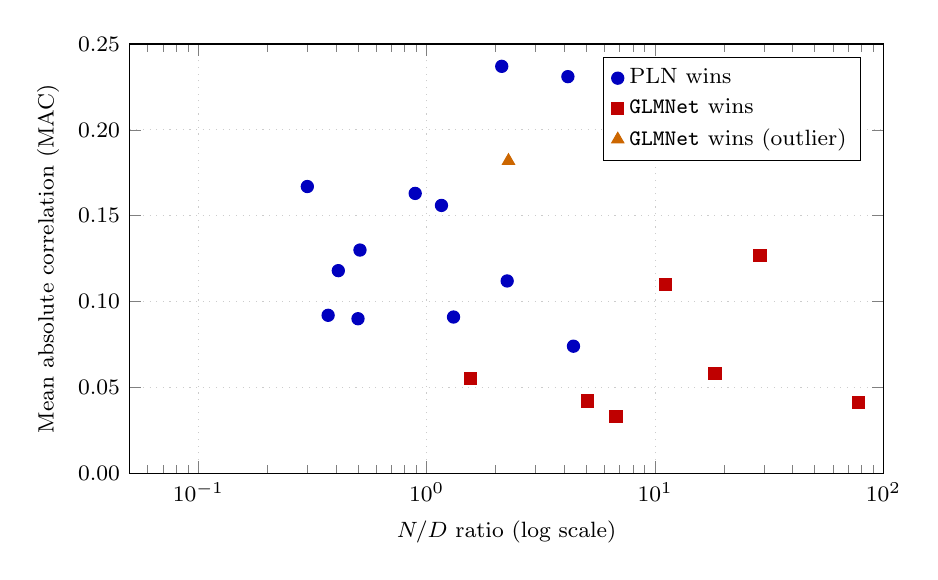
\begin{tikzpicture}
\begin{axis}[
  width=0.92\textwidth,
  height=0.58\textwidth,
  xlabel={$N/D$ ratio (log scale)},
  ylabel={Mean absolute correlation (MAC)},
  xmode=log,
  xmin=0.05, xmax=100,
  ymin=0, ymax=0.25,
  ytick={0, 0.05, 0.10, 0.15, 0.20, 0.25},
  yticklabel style={/pgf/number format/fixed, /pgf/number format/fixed zerofill,
                    /pgf/number format/precision=2, font=\footnotesize},
  ymajorgrids=true,
  xmajorgrids=true,
  grid style={dotted, gray!40},
  tick label style={font=\footnotesize},
  label style={font=\footnotesize},
  legend style={font=\footnotesize, at={(0.97,0.97)}, anchor=north east},
  legend cell align=left,
]
\addplot[only marks, mark=*, mark size=2.2pt, blue!75!black]
  coordinates {
    (0.30,0.167)(0.37,0.092)(0.41,0.118)(0.50,0.090)
    (0.51,0.130)(0.89,0.163)(1.16,0.156)(1.31,0.091)
    (2.13,0.237)(2.25,0.112)(4.15,0.231)(4.39,0.074)
  };
\addlegendentry{PLN wins}
\addplot[only marks, mark=square*, mark size=2.2pt, red!75!black]
  coordinates {
    (1.56,0.055)(5.07,0.042)(6.74,0.033)(11.08,0.110)
    (18.30,0.058)(28.80,0.127)(77.74,0.041)
  };
\addlegendentry{\texttt{GLMNet} wins}
\addplot[only marks, mark=triangle*, mark size=2.5pt, orange!80!black]
  coordinates {
    (2.28,0.182)
  };
\addlegendentry{\texttt{GLMNet} wins (outlier)}
\end{axis}
\end{tikzpicture}
\end{center}
